\documentclass[conference]{IEEEtran}
\IEEEoverridecommandlockouts
% The preceding line is only needed to identify funding in the first footnote. If that is unneeded, please comment it out.
\usepackage{cite}
\usepackage{amsmath,amssymb,amsfonts}
\usepackage{algorithmic}
\usepackage{graphicx}
\usepackage{textcomp}
\usepackage{xcolor}

\def\BibTeX{{\rm B\kern-.05em{\sc i\kern-.025em b}\kern-.08em
    T\kern-.1667em\lower.7ex\hbox{E}\kern-.125emX}}
\begin{document}

\title{Dashcam for Traffic Object Detection\\ }

\makeatletter
\newcommand{\linebreakand}{%
  \end{@IEEEauthorhalign}
  \hfill\mbox{}\par
  \mbox{}\hfill\begin{@IEEEauthorhalign}
}
\makeatother

\def\Affiliation{ School of Electrical Engineering }
\def\Organization{Telkom University, Indonesia}
\def\CityCountry{Bandung, Indonesia}

\author{\IEEEauthorblockN{Aura Syafa Aprillia Radim}
\IEEEauthorblockA{\textit{\Affiliation} \\
\textit{\Organization}\\
\CityCountry \\
syafaaura@student.telkomuniversity.ac.id }
\and
\IEEEauthorblockN{Muchammad 'Irfan Chanif Rusydi}
\IEEEauthorblockA{\textit{\Affiliation} \\
\textit{\Organization}\\
\CityCountry \\
chanifrusydi@student.telkomuniversity.ac.id}
\and
\IEEEauthorblockN{Surya Michrandi Nasution}
\IEEEauthorblockA{\textit{\Affiliation} \\
\textit{\Organization}\\
\CityCountry \\
email address or ORCID}
\linebreakand
% \IEEEauthorblockN{4\textsuperscript{th} Given Name Surname}
% \IEEEauthorblockA{\textit{dept. name of organization (of Aff.)} \\
% \textit{name of organization (of Aff.)}\\
% City, Country \\
% email address or ORCID}
% \and
\IEEEauthorblockN{Casi Setianingsih}
\IEEEauthorblockA{\textit{\Affiliation} \\
\textit{\Organization}\\
\CityCountry \\
email address or ORCID}
% \and
% \IEEEauthorblockN{6\textsuperscript{th} Given Name Surname}
% \IEEEauthorblockA{\textit{dept. name of organization (of Aff.)} \\
% \textit{name of organization (of Aff.)}\\
% City, Country \\
% email address or ORCID}
}

\maketitle

\begin{abstract}
Dashcam is a camera place on dashboard  in vehicle. This tool serves to record all events in front of the vehicle. 
Security and safety have become a major concern in various sectors, including transportation and public security. 
On the highway, traffic accidents caused by the driver's ignorance of objects around the vehicle are still a serious problem. 
In this study, the development of a simple dashcam built from an edge computer was carried out by combining the number of cameras. Image stitching is applied to combine images that have been collected by each camera.  
Next, object detection is carried out on the images that have been collected. The object detection system approach is carried out using YOLOv8 which is the latest variant of the YOLO series. This research is expected to be one step in the development of an Intelligent Transportation System that is in accordance with traffic conditions in Indonesia.
The results obtained in testing using the system created exist using the configuration of 78,000 datasets, 3332 data validation with 8 epochs, batch size 32, linear learning rate and SGD optimization. Results are best in the morning and afternoon. The program can recognize predefined objects. 
\end{abstract}

\begin{IEEEkeywords}
object detection, YOLOv8, dashcam
\end{IEEEkeywords}

\section{Introduction}
% bahas dashcam, YOLO 8, sekarang ini banyak yang memakai dashcam, tapi dashcam yang ada sekarang hanya untuk merekam, belum ada yang bisa mendeteksi objek di depannya
Security and safety have become a major concern in various sectors, including transportation and public security. On the highway, traffic accidents caused by the driver's ignorance of objects around the vehicle are still a serious problems
Smart and effective object detection technology is becoming increasingly important for monitoring traffic [1].

Dashcam is a camera placed on the dashboard of a vehicle. This device usually serves to record all events in front of the vehicle.
Dashcam is one of the devices that the demands is growing rapidly in the market. Currently, dashcam serves as a device to record events in front of the vehicle and then the recording is used as evidence in the event of an accident or proof of insurance claims. 
However, dashcam could also be used for other purposes, such as being used as one of the components of an Autonomous Driving Assistance System (ADAS). 

In this paper, we propose a simple solution to prevent accidents amongs vehicles. Our solution is by implementing object detection and single board computer (SBC) as processing unit. Object in front of the camera can be detected by Convolutional Neural Network. 
The content of this paper is organized as follows. Section 2 presents the literature review. Section 3 presents the system design. Section 4 presents our experimentaton in the process of developing the system. Section 5 presents the conclusion and future work.

\section{Literature Review}
\subsection{Dashcam}
% Masukin litarasi dashcam, terakhir masukin related work monocular raspbberry pi
Both China and South Korea governments obliges public transportation and commercial vehicles to install dashcam in order to assist the investigation of traffic accidents\cite{Korea Dashcam}.


\subsection{Object Detection}
Object Detection is one of the important task in computer vision field, mainly dealing with detecting instances of visual object then categorize them into several classes \cite{b2}.
With this kind of identification and localization, object detection can be used to count objects in a scene and determine and track their precise locations, all while accurately labeling them.
Object detection has been widely used for face detection, vehicle detection, pedestrian counting, web images, security systems and driverless cars.
Within the past twenty years, object detection have been going through a lot of changes and development. Although it is commonly divided into two periods: "traditional object detection" and "deep learning based".
In 2012, Krizhevsky et al.~\cite{b3} proposed a deep convolutional network trained on a subset of ImageNet. 

This network, called AlexNet, was 
A year later, Girshick et al. \@ proposed a new object detection framework called R-CNN~\cite{b4} because it used region proposals combined with CNNs to detect objects in images.

Since then, the field of object detection has been rapidly advancing, with new models, datasets, and techniques emerging in a rapid pace. 

\subsection{YOLO}
%tambahkan gambar atau ilustrasi CNN atau YOLO 
With the born of AlexNet, YOLO (You Only Look Once) model was introduced in 2015. Original base YOLO model can achieve 45 frame per second.
While the sameller version, Fast YOLO can achieve 155 frames per second.
YOLO outperform DPM and R-CNN on Picasso Dataset and People-Art Dataset~\cite{You Only Look Once}.

In the early period of making this paper, YOLOv7 was the latest version of YOLO\@.
However,as January 2023, YOLOv8 was introduced by Ultralytics, the same software company that release YOLOv3 and YOLOv5. 
As of now,YOLOv8 is one of the latest State of The Art (SOTA) open source object detection model. Following its predecessor, YOlov8 offers several model size.
From the YOLOv8n as the smallest model, YOLOv8l as the medium model, and YOLOv8x as the largest model.
We choose YOLOv8n as our model because it is the smallest model and can be run on edge computer.
YOLOv8n have x parameters. With computation cost around 8 GFLOPs.
\subsection{COCO Dataset}\label{AA}
The COCO dataset is a large-scale object detection, segmentation, and keypoint dataset.
In total, The Microsoft Common Objects in COntext contains 91 common object categories with 82 of them having more than 5,000 labeled instances~\cite{COCO Dataset}.
The first release of COCO Dataset was in 2014. In 2014, COCO Dataset has 83,000 image in train split and 41,000 image in validation split.
After taking community feedback, COCO Dataset increase total number of images and changes its split proportion. In 2017 release, train2017 split have 118,000 image files and 5,000 images in val2017 split.
Given its size, COCO Dataset widely used by tate of the Art Object Detection Model to train and eveluate the model performance.

Despite its popularity, COCO Dataset has some drawbacks. COCO Dataset contains 80 classes. However, COCO Dataset have imbalance class distribution.
For example, the number of person class is 64115, while the number of hair drier class is only 100.
\begin{figure}[h]
\centering
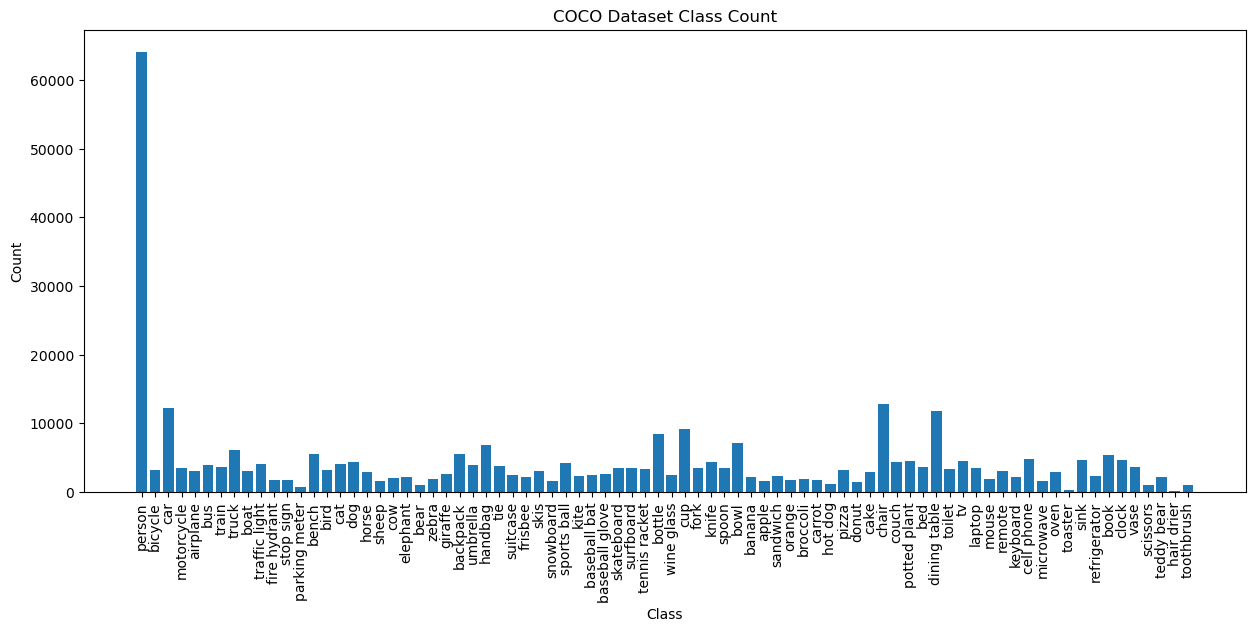
\includegraphics[width=0.5\textwidth,keepaspectratio]{coco_class_count.png}
\caption{COCO Dataset Class Count}
\end{figure}

\subsection{Filtering Dataset}\label{Filtering}
As mention earlier, COCO dataset contains 80 classes. However, we only need traffic related object classes.
Therefore, we filtered the dataset to only contains 12 classes. The classes are:
Car Truck Bus Motorcycle Bicycle Traffic Light Stop Sign Train Hydrant Cat Dog
The result is 78,663 images in training split with 12 classes. This amount of data was reduced from 122,125 images in original dataset. By reducing the dataset, our model expected to take less time to train.
\begin{figure}[h!]
\centering
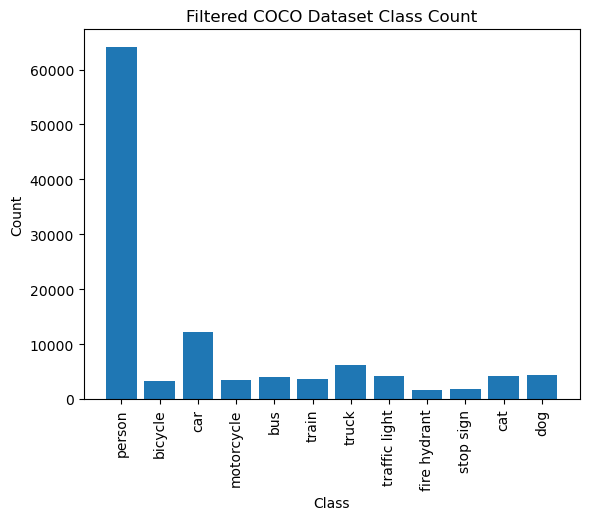
\includegraphics[width=0.5\textwidth,keepaspectratio]{filtered_coco_class_count.png}
\caption{Filtered COCO Dataset Class Count}
\end{figure}

\begin{figure}[h!]
\centering
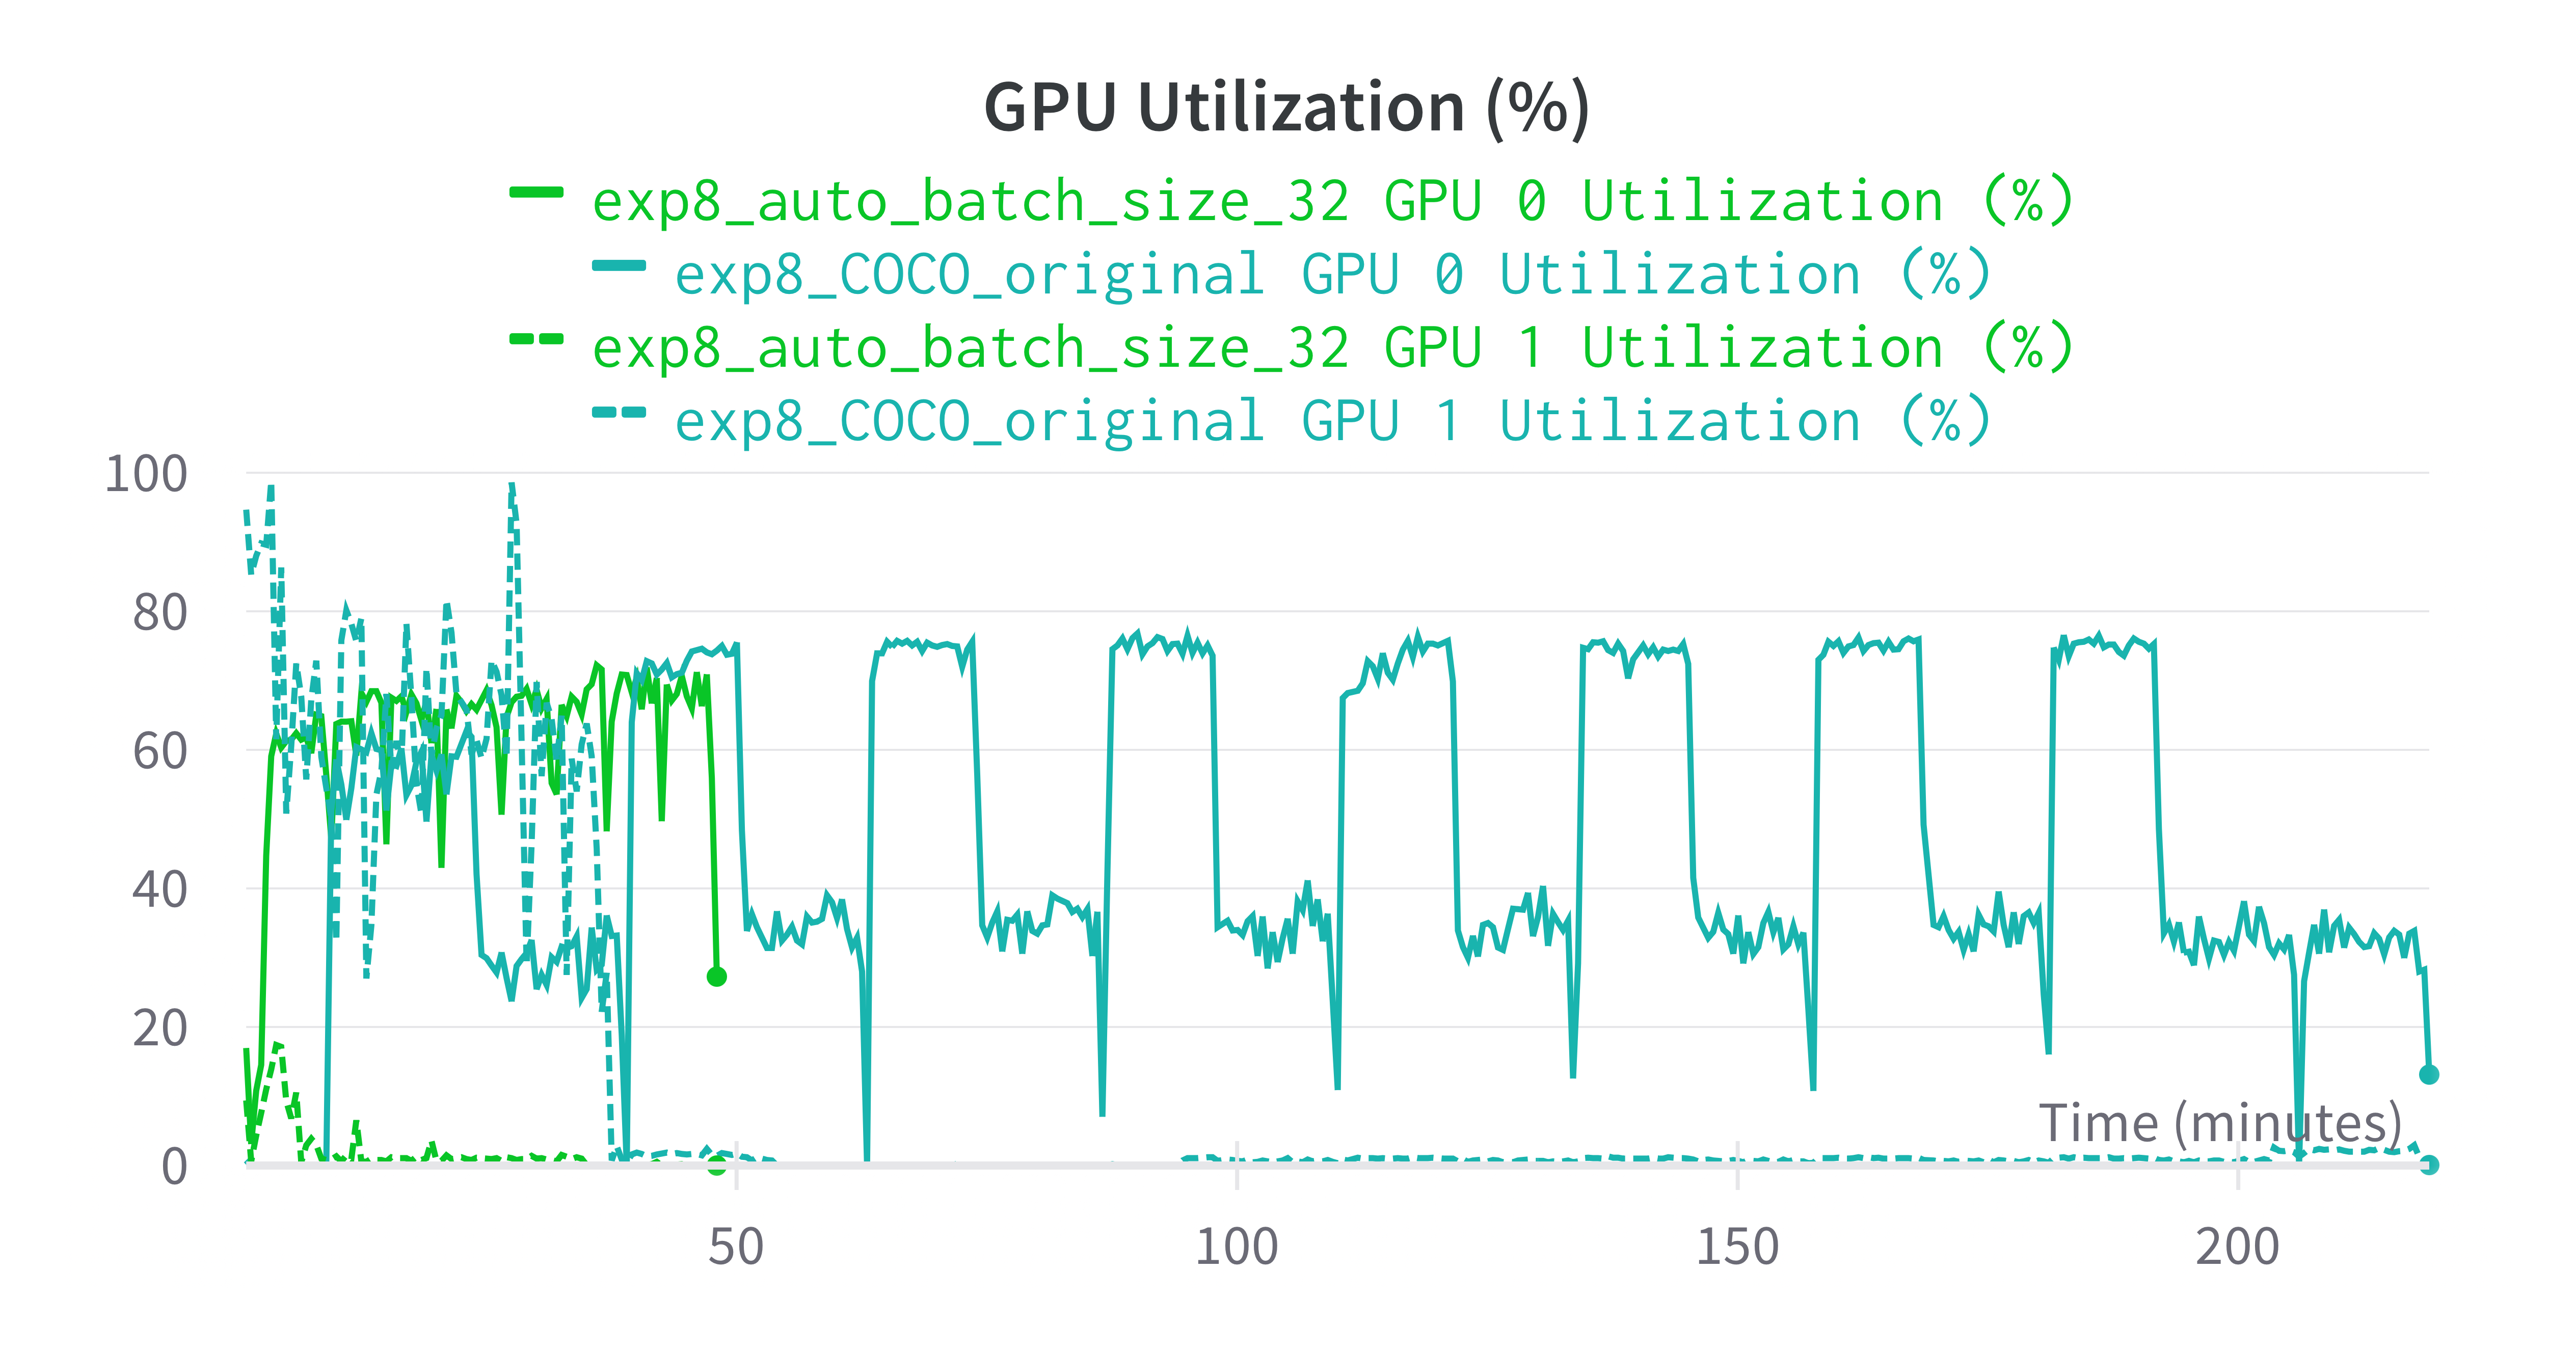
\includegraphics[width=0.3\textwidth,keepaspectratio]{gpu_utilization_comparison_original_and_filtered.png}
\caption{Comparison of GPU Utilization between training the model using filtered dataset and original dataset}
\label{fig:original_filtered_gpu_utilization}
\end{figure}

\begin{figure}[h!]
\centering
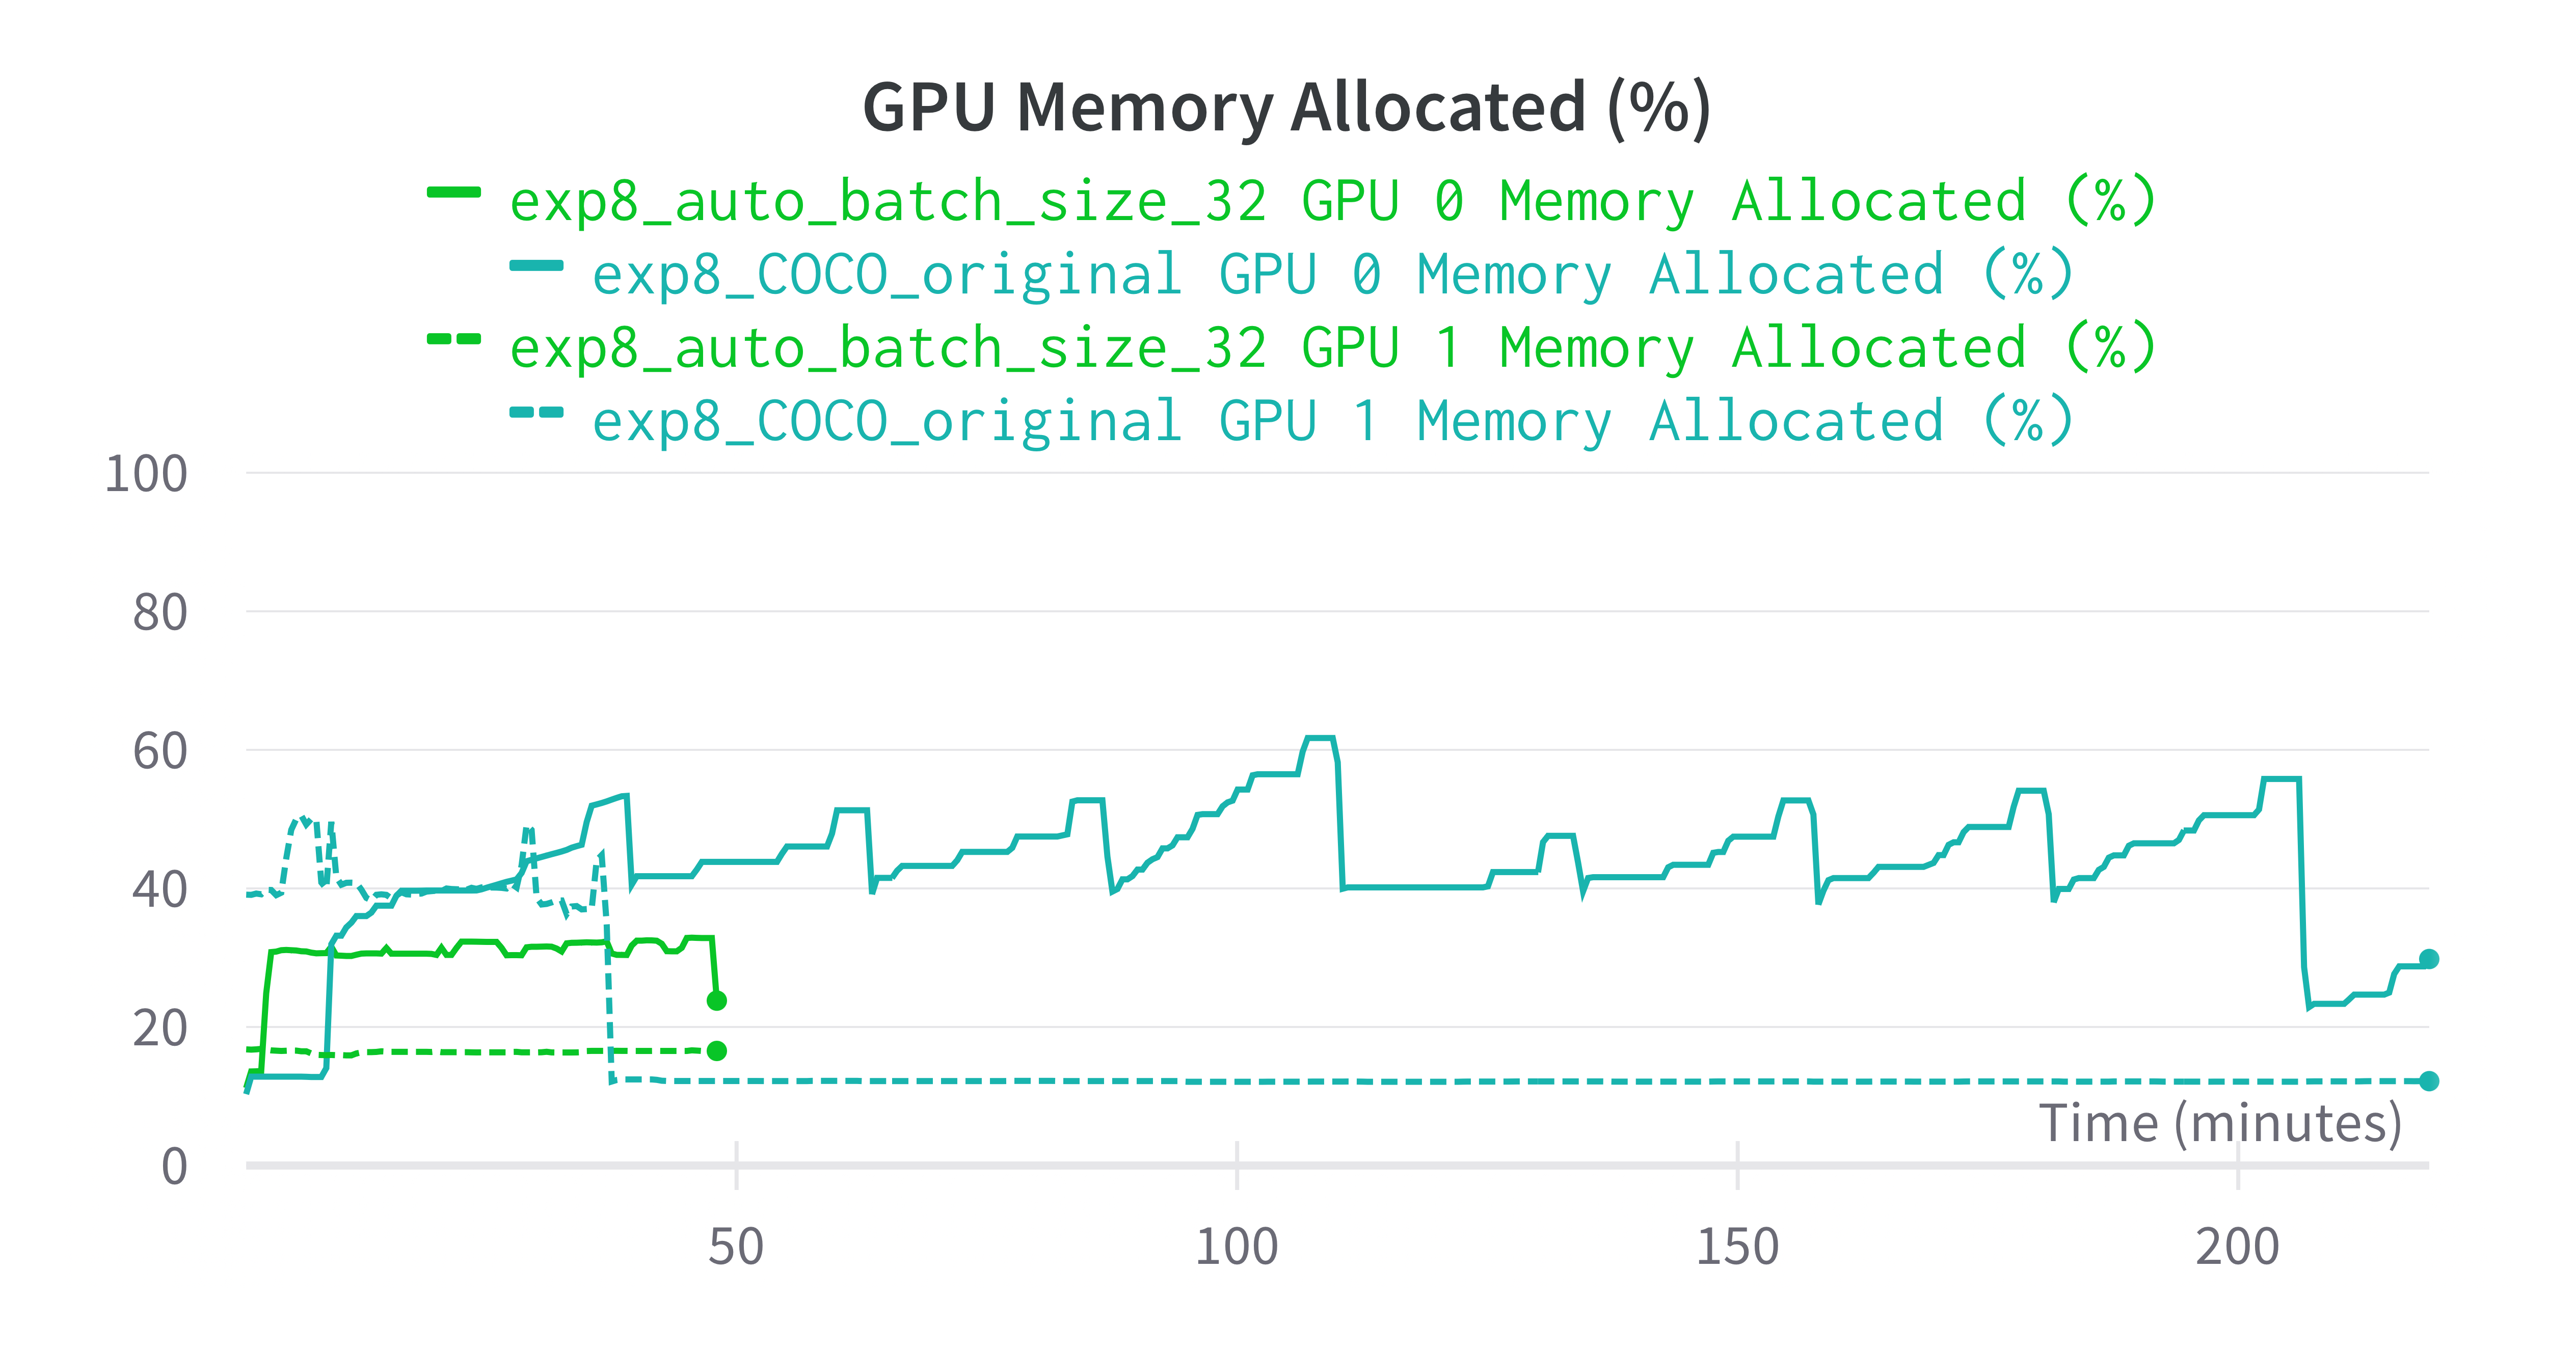
\includegraphics[width=0.3\textwidth,keepaspectratio]{memory_utilization_comparison_original_and_filtered.png}
\caption{Comparison of GPU Memory Utilization between training the model using filtered dataset and original dataset}
\label{fig:original_filtered_memory_utilization}
\end{figure}
In addition, as shown in Fig. \ref{fig:original_filtered_gpu_utilization} and Fig.\ref{fig:original_filtered_memory_utilization}, the filtered dataset has lower GPU Utilization and Memory Utilization. This means that the filtered dataset is more efficient to train.
Thus allowing us to push model training further.
Metrics wise, the model trained using filtered dataset showed better result.

\subsection{Performance Metrics}
For training and validation purposes, we focus on mAP (mean Average Precision), Precision, and recall. mAP is the average of AP (Average Precision) over all classes. AP is the area under the precision-recall curve.
We compare mAP averaged for IoU (Intersection over Union) thresholds from .50 to .95 with .05 increments (MS COCO standard metric, abbreviated as mAP50-95) and mAP50 (PASCAL VOC metric, abbreviated as mAP50) \cite{b7}. 
Precision and Recall in  this experiment is a relative measure, because it depends on the threshold value.
Precision calculated by dividing True Positive by the sum of True Positive and False Positive. 
Precision is calculated using \eqref{equation1}.
\begin{equation}
Precision = \frac{TP}{TP+FP}
\label{equation1}
\end{equation}
Recall calculated by dividing True Positive by the sum of True Positive and False Negative.
\begin{equation}
Recall = \frac{True Positive}{TruePositive+FalseNegative}
\end{equation}
Threshold value determines whether the prediction is Positive or Negative. For example, if the threshold is 0.5, then the prediction is positive if the IoU is greater than 0.5. Otherwise, the prediction is negative.

Both Precision and Recall are relative to the threshold value and usually used in the form of Precision-Recall Curve. We can calculate the area under the curve to get the Average Precision
To get the value of mAP, we need to calculate Average Precision for each class. Then, we calculate the mean from all Average Precision we calculate earlier.
\begin{equation}
mAP = \frac{1}{n}\sum_{i=1}^{n}AP_i
\label{mAP}
\end{equation}
$\eta$ is the number of classes.
This is the main reason of filtering Dataset would be beneficial in our training process. As we use filtered dataset, the value of $\eta$ in equation \ref{mAP} is 12 instead of 80.
Figure 3 shows the comparison of mAP50 and mAP50-95 between training the model using filtered dataset and original dataset. We can see that the filtered dataset has better mAP50 and mAP50-95 than original dataset.



\section{System Design}
% Flowchart di sini aja
% Fig 1 ceritakan lebih detail
% cerita singkat kita implementasi di jetson nano

Nasution and Dirgantara system
\section{Experiments}


\subsection{Experimental Setup}
In this section, we will discuss about the experimental setup. We are using Pytorch as our deep learning framework in Python  3.
MNodel training was conducted on Geforce RTX 3090, 24 GB VIdeo RAM, 32GB RAM, Intel Core i3-12100 4 Core 8 Thread, running on Windows 10
Model inference and testing was performed on Macbook Air M1, and Jetson Nano 4GB. The camera used in this experiment is Lifecam Studio by Microsoft.
Jetson Nano that we use running on Ubuntu 20.04.2 LTS on top of Jetpack 4.6. We use Jetson Nano 4GB as our edge computer because it is the most affordable edge computer in Nvidia Jetson Series.
\subsection{Testing Dataset}
As mention earlier, we are using COCO dataset. However, we filtered the dataset to only contain 12 classes. The classes are:
Car, Truck, Bus, Motorcycle, Bicycle, Traffic Light, Stop Sign, Train, Hydrant, Cat, Dog. The result is 78000 images with 12 classes.
For inference and real world testing, we gather our own data by recording traffic condition in Bandung, Indonesia. The data was recorded using camera mentioned earlier.

\subsection{Training}
Before we begin training process of our YOLOv8n-Traffic model with high number of epoch, we want to find the optimal hyperparamater configuration for our use case. We conducted various training configuration with 8 epoch to save time.
Although each run for one configuration is only 8 epoch, it's still takes about 1 to 2 hours. However, we can get the result faster than training with 100 epoch for each configuration.

We tried different batch size, learning rate, and optimizer. We use batch size 16 and 32.
\begin{figure}[h]
\centering
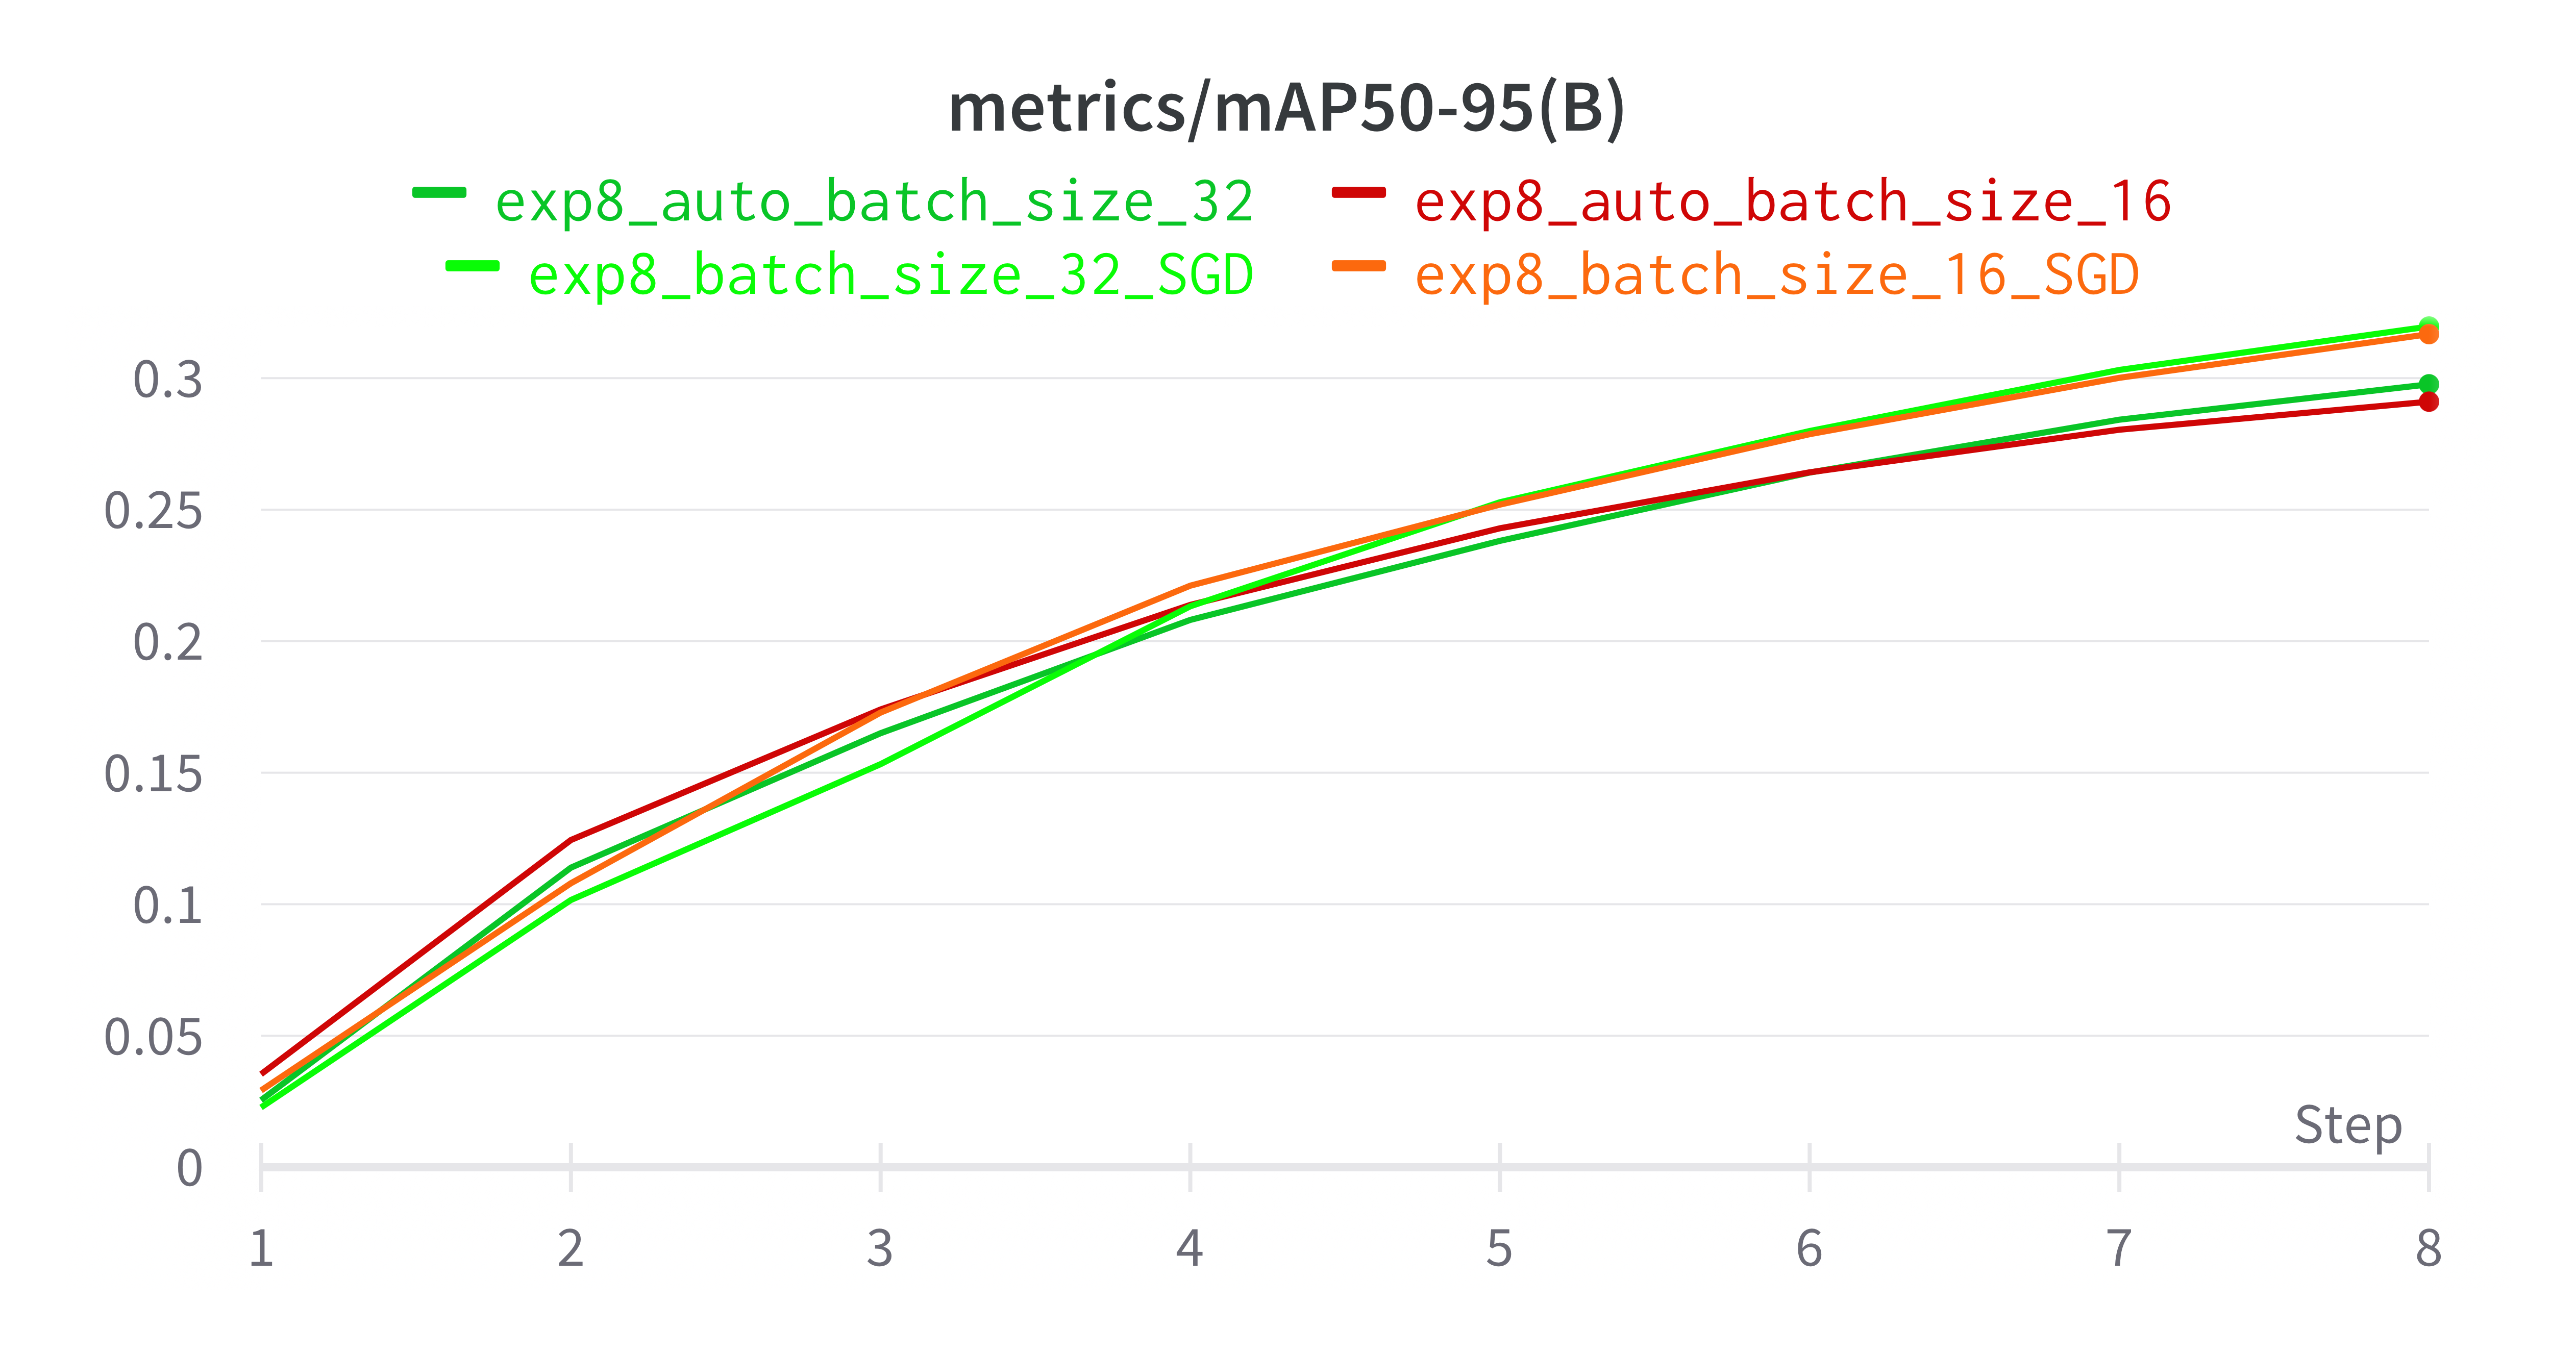
\includegraphics[width=0.3\textwidth,keepaspectratio]{mAP_batch_size_comparison.png} % TODO ; change file name
\caption{Comparison of mAP50-95 between training the model using batch size 16 and 32}
\label{fig:batch_size}
\end{figure}

\begin{figure}[h!]
\centering
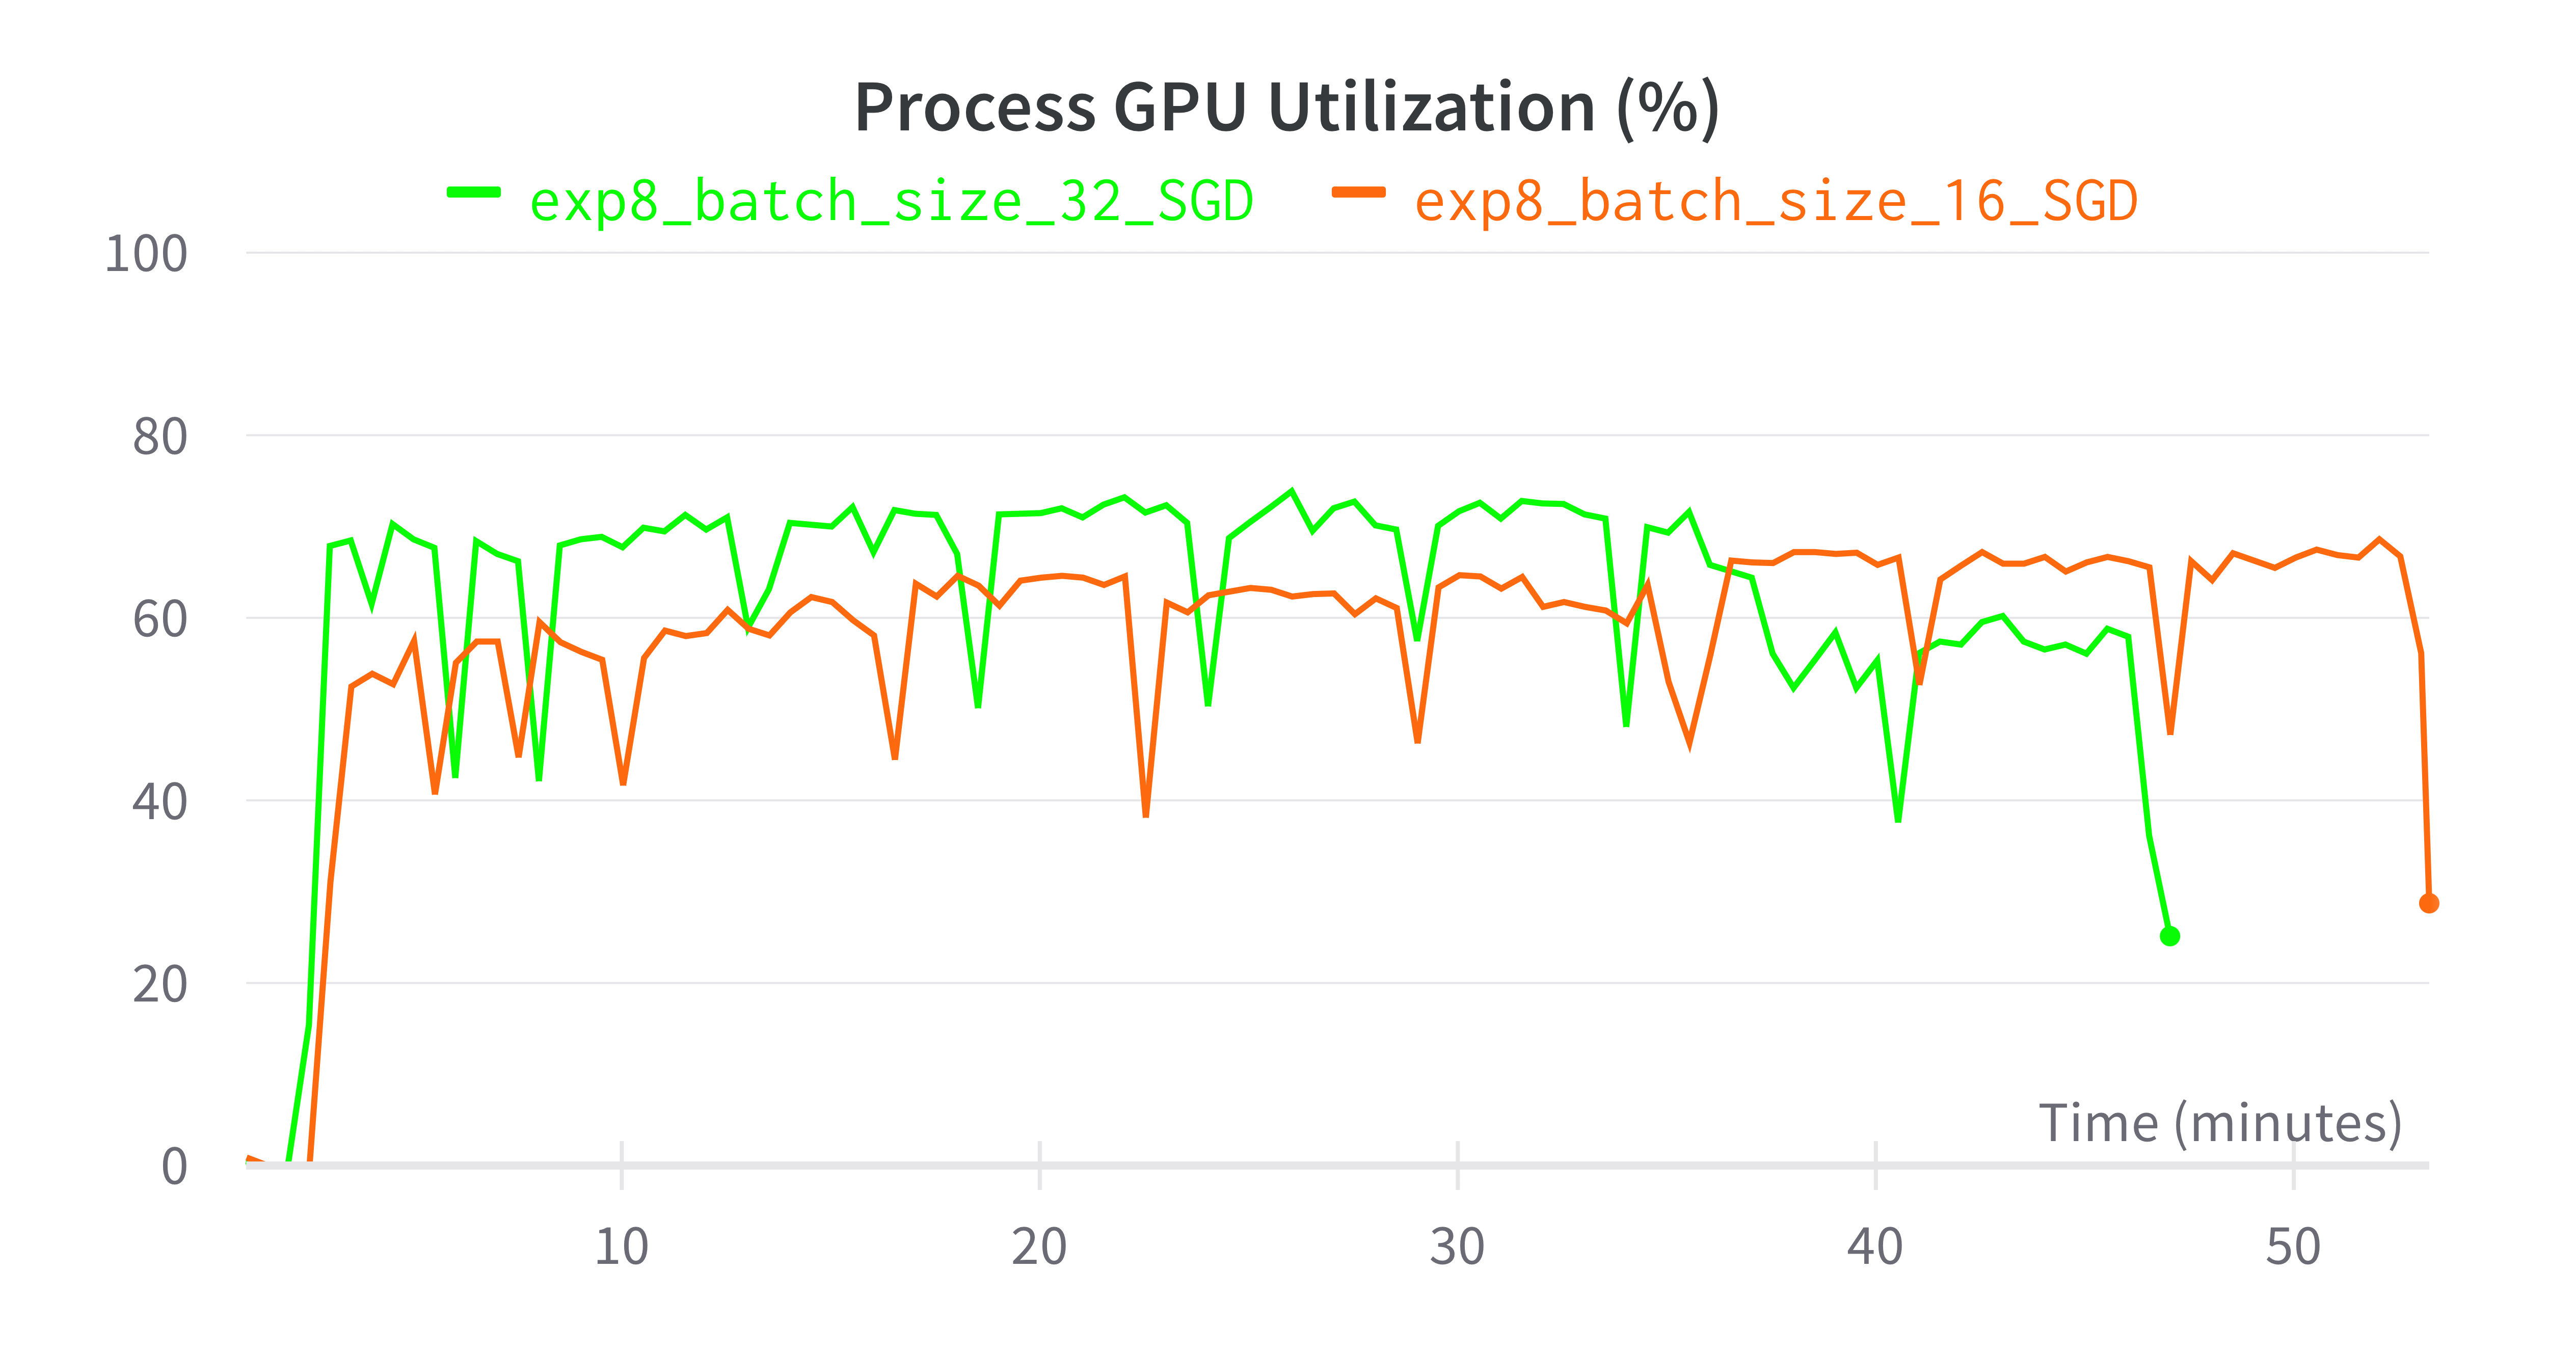
\includegraphics[width=0.3\textwidth,keepaspectratio]{gpu_utilization_comparison.png} 
\caption{Comparison of GPU Utilization between training the model using batch size 16 and 32}
\label{fig:gpu_utilization}
\end{figure}
% gpu_utilization_comparison.png
Fig.\ref{fig:batch_size} shows the result of training with different batch size. We can see that batch size 32 is better than batch size 16. Especially in terms of training time, batch size 32 is faster than batch size 16.
Therefore, we use batch size 32 for our training. We also tried using SGD and Adam optimizer. YOlOv8 implement optimizer switching depends on the number of iterations.




\subsection{Real World Testing}
In this section, we will discuss about the real world testing. We bring our system to real world environment scenario, placed our whole system into the dashboard of vehicles.
\begin{figure}[h!]
    \centering
    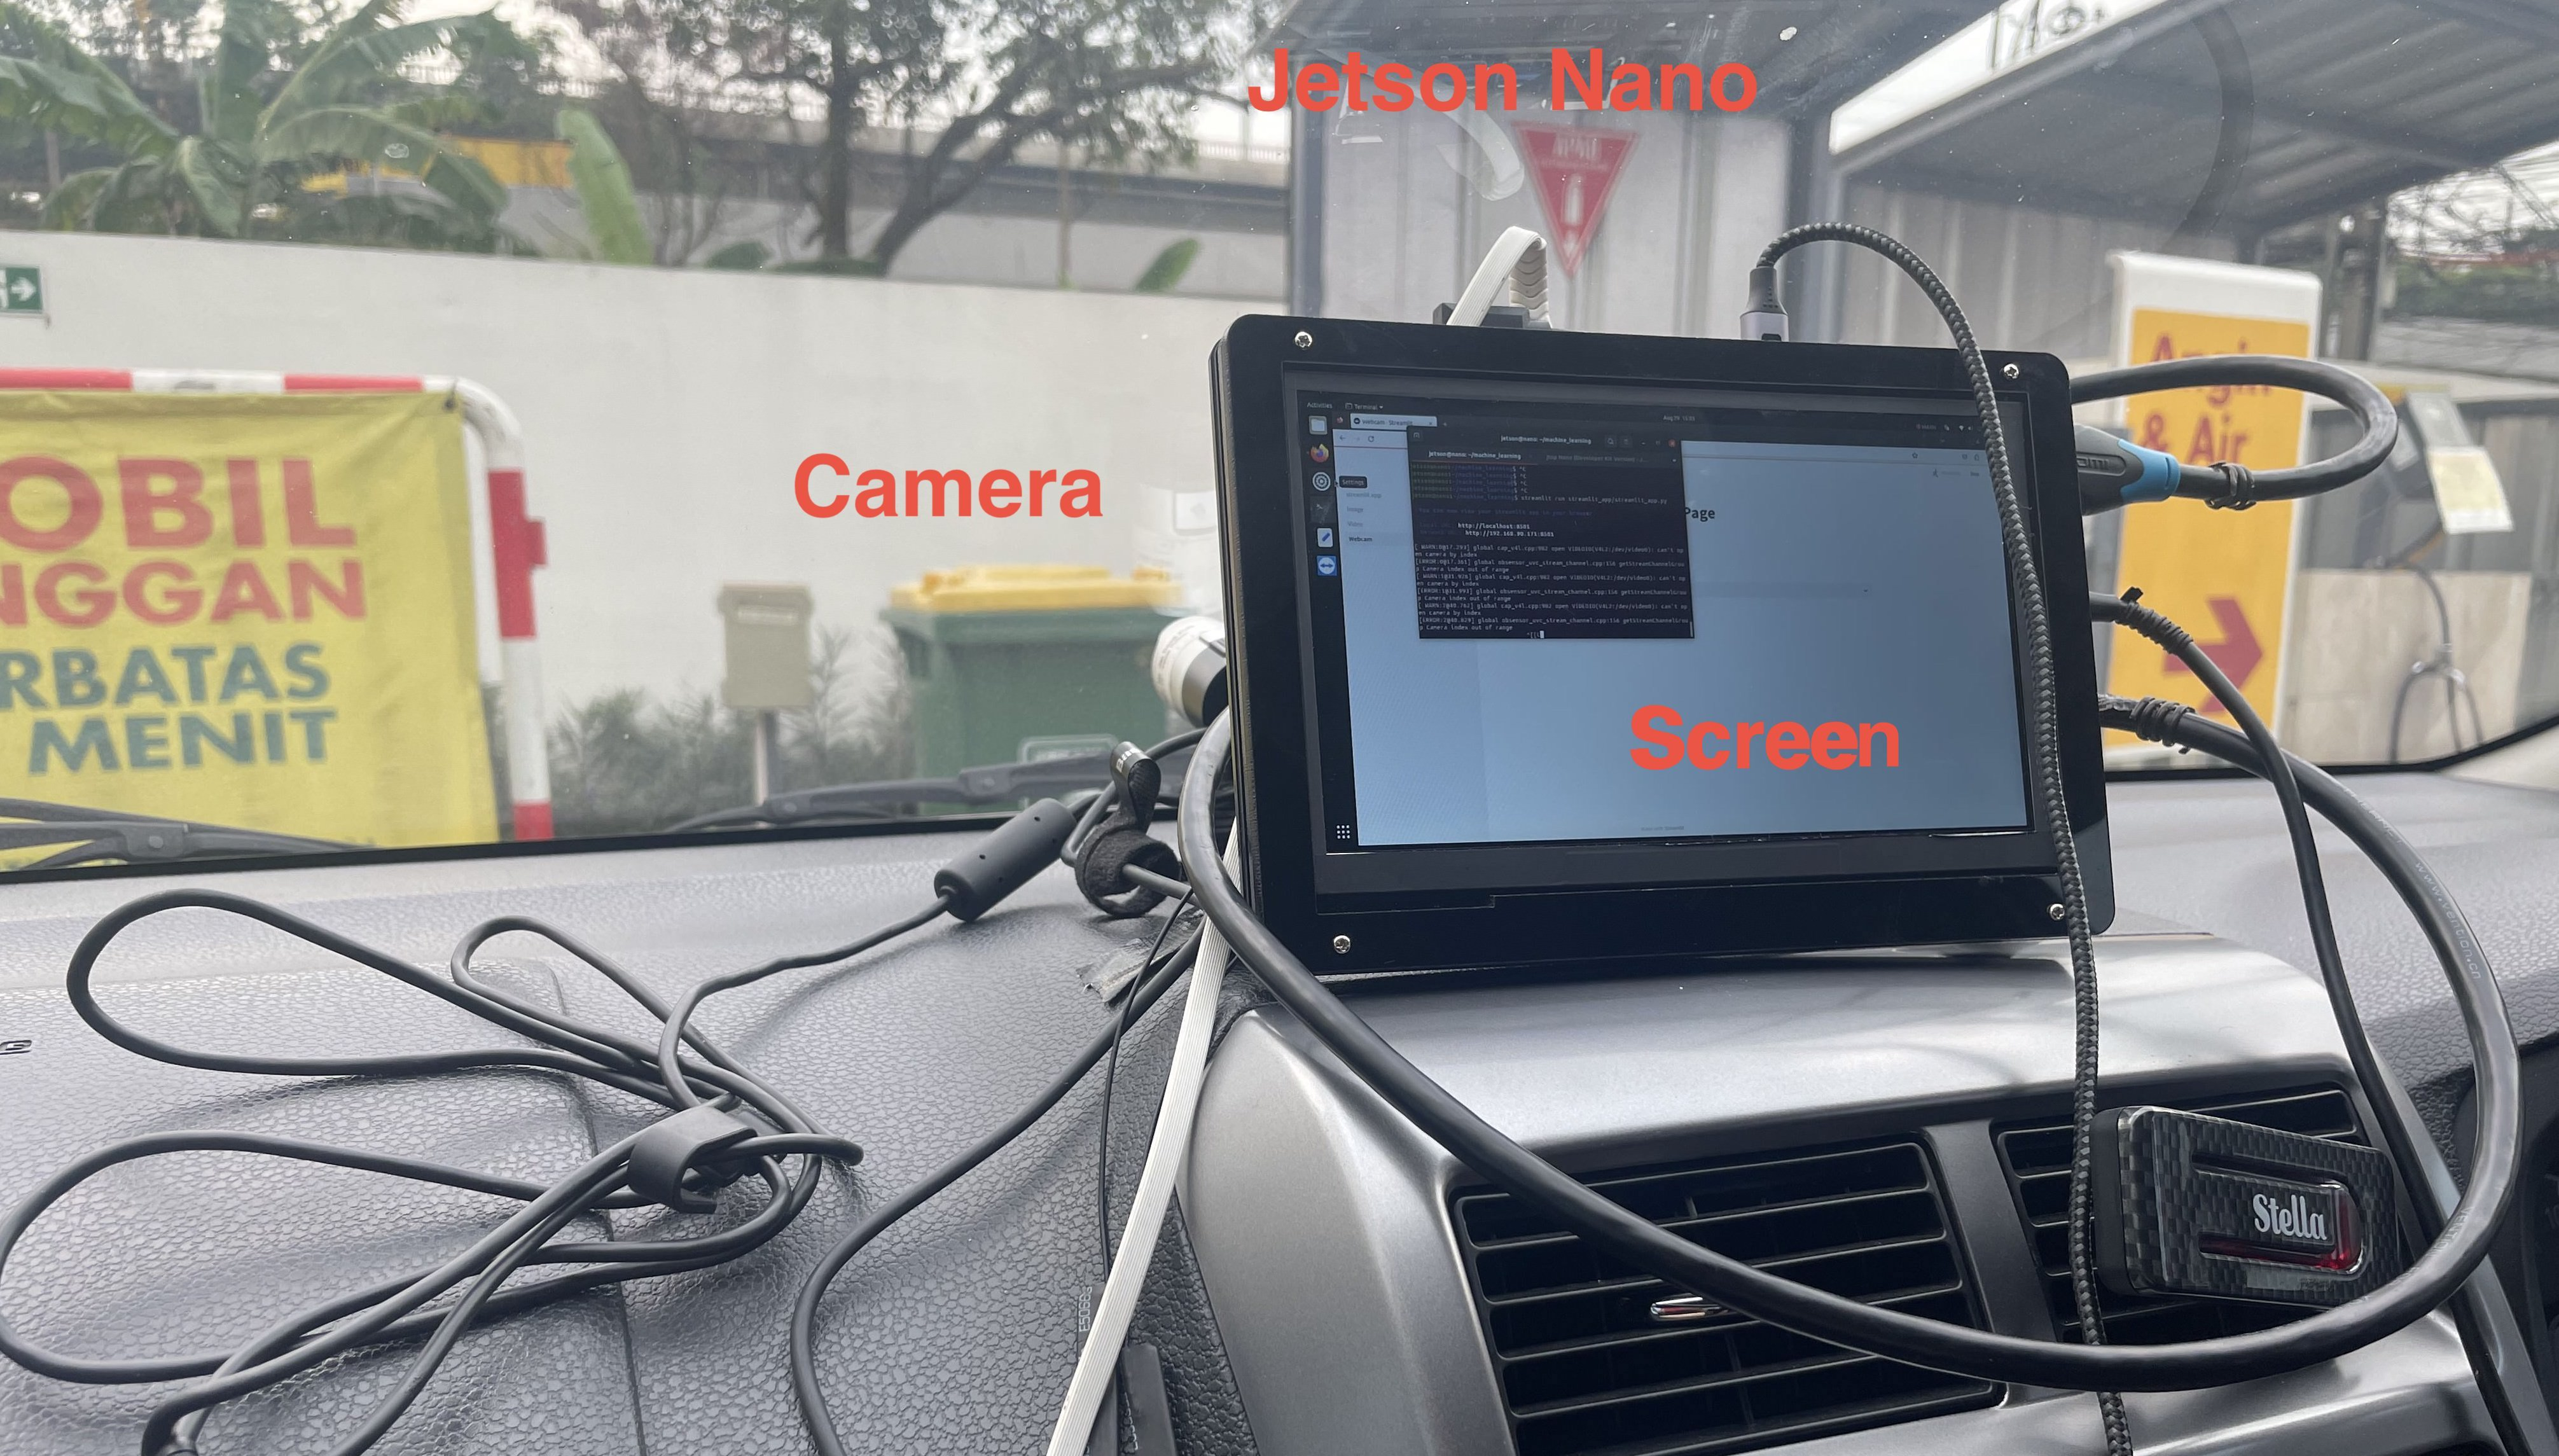
\includegraphics[width=0.4\textwidth,keepaspectratio]{mounted_camera_front_view.jpg}
    \caption{Front View}
    \label{fig:front_view}
\end{figure}

\begin{figure}[h!]
    \centering
    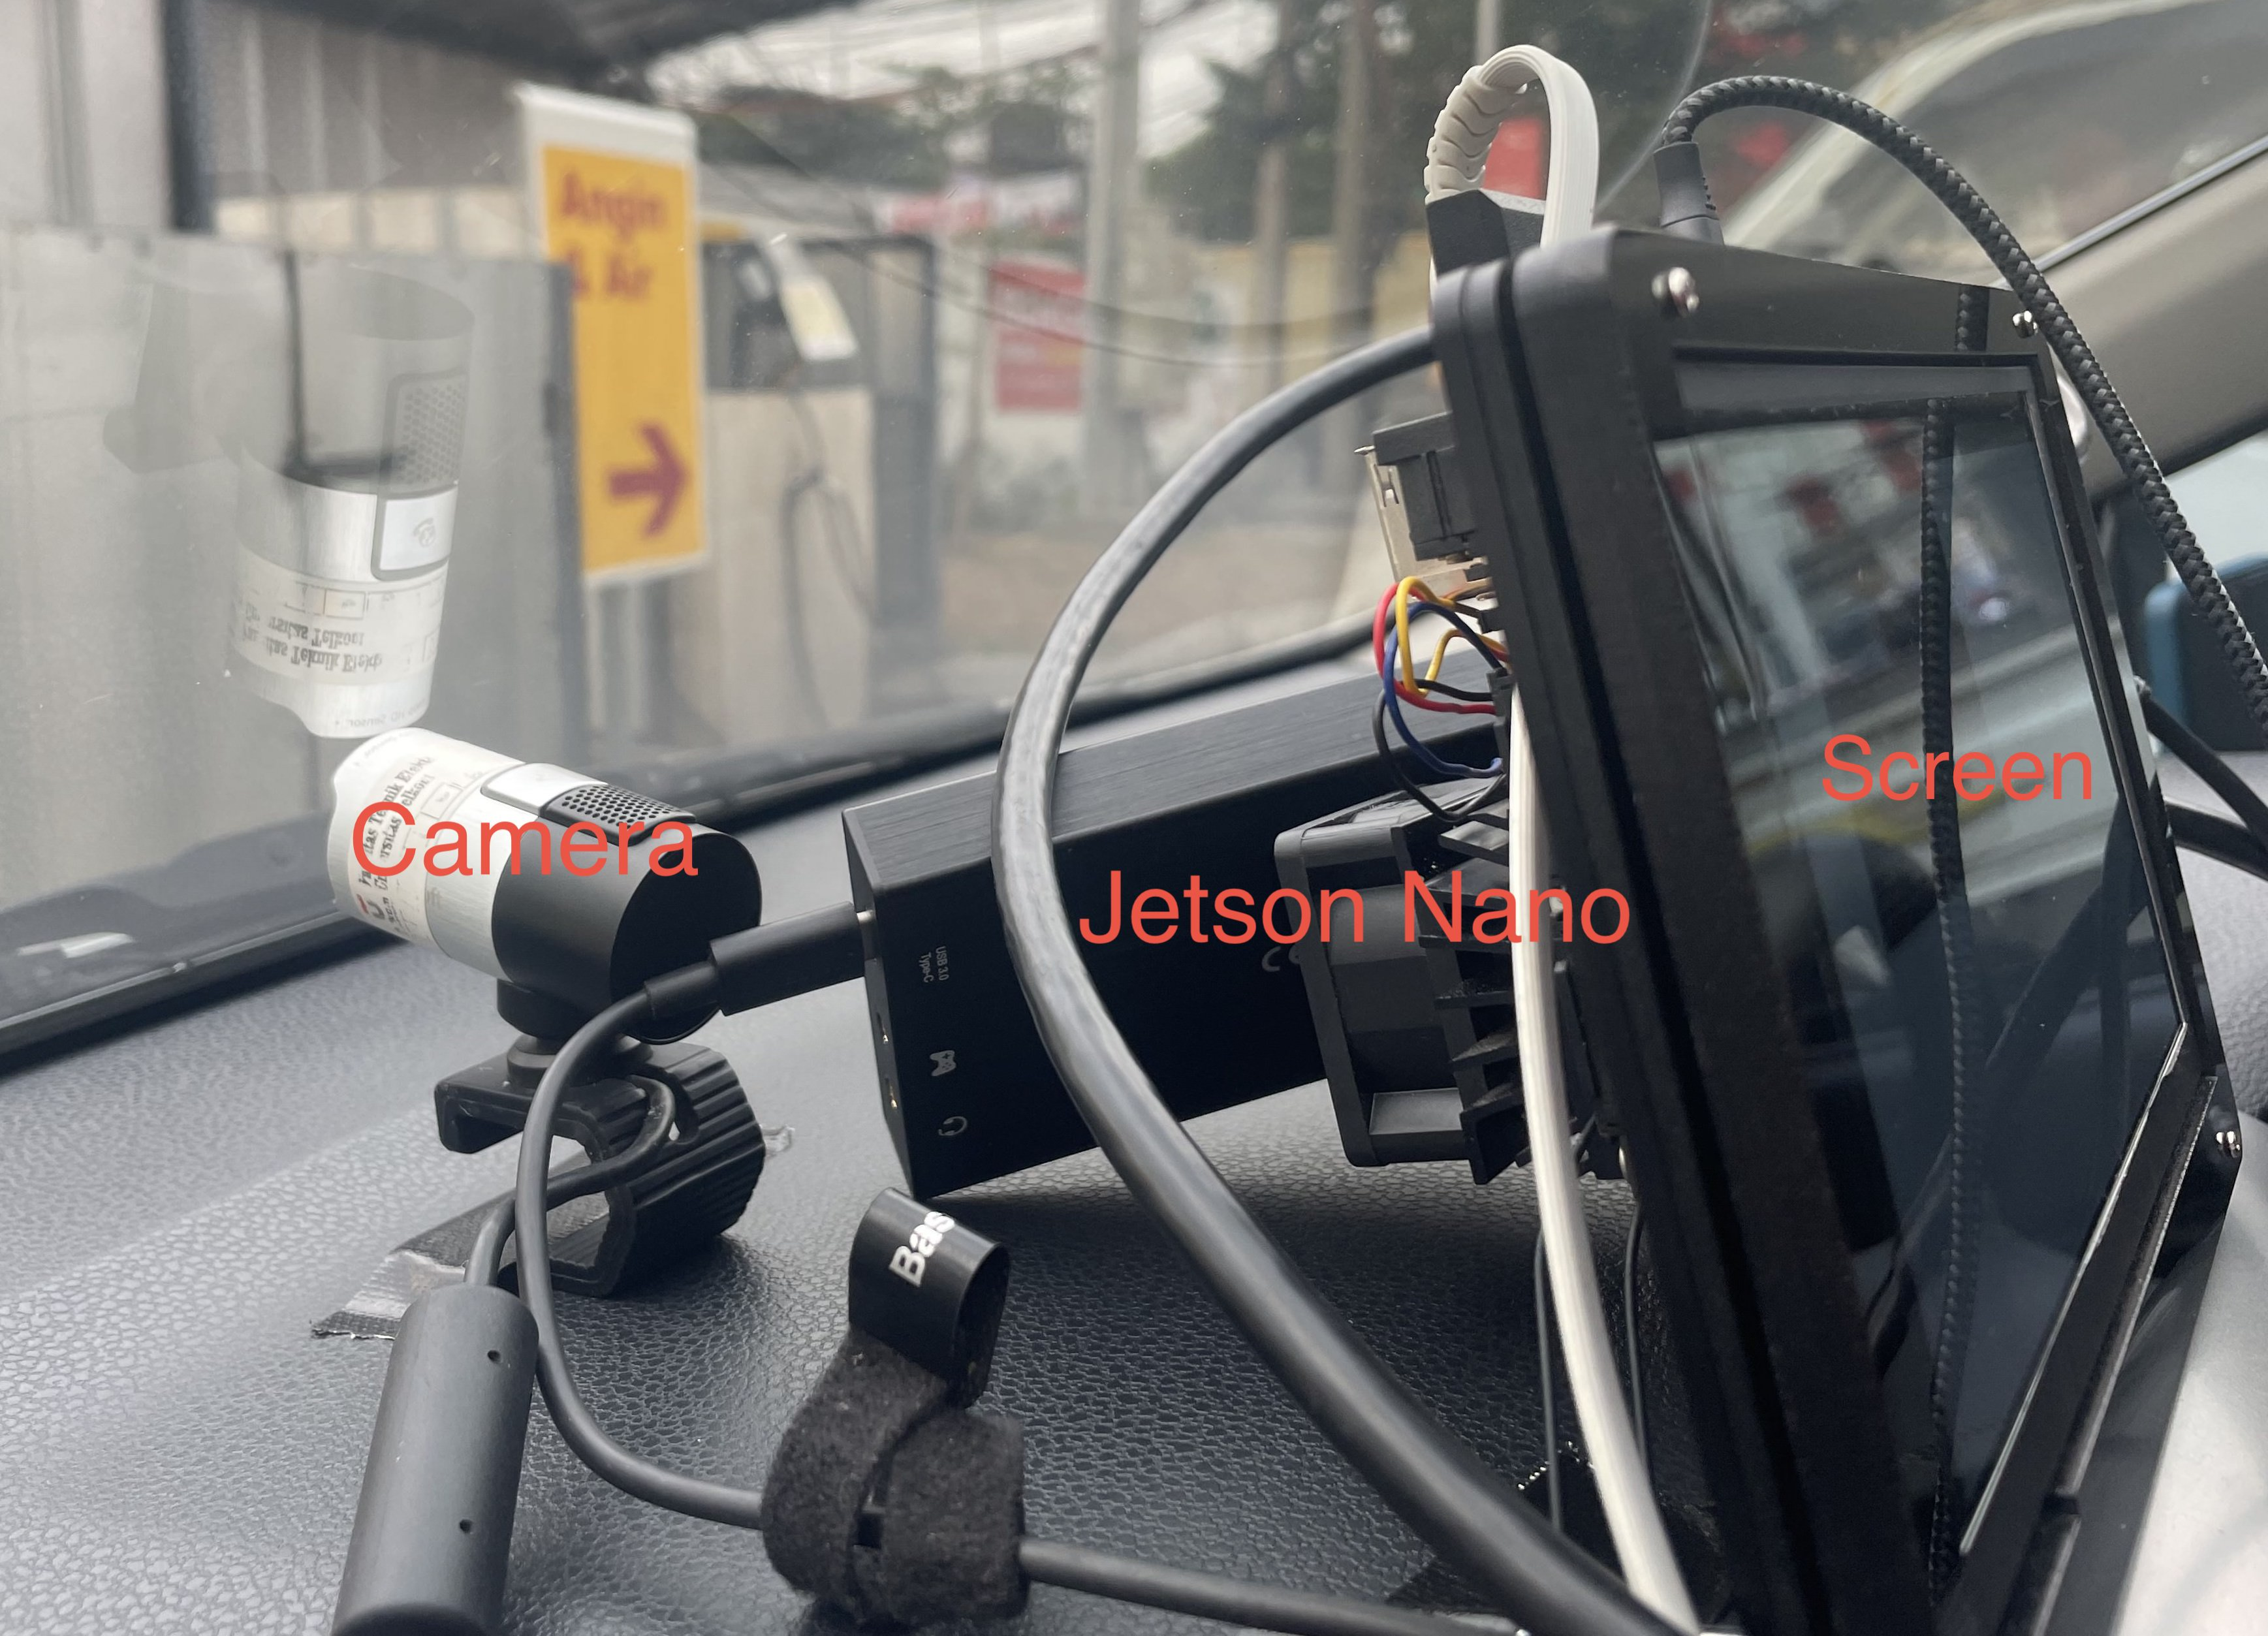
\includegraphics[width=0.4\textwidth,keepaspectratio]{mounted_camera_side_view.jpg}
    \caption{Side View}
    \label{fig:side_view}
\end{figure}


\section{Results and Discussion}
In this section, we will discuss about the result of our experiment. We will discuss about the result of training and real world testing.
\subsection{Training Result}
In this section, we will discuss about the result of our training. In order to compare the performance of YOLOv8n model, we also train YOLOv7-tiny model.

\begin{figure}[h!]
\centering
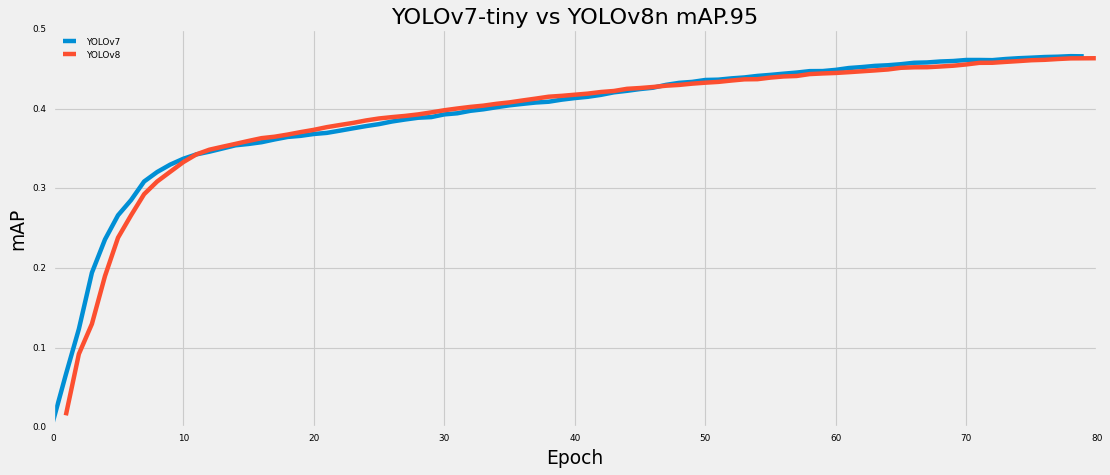
\includegraphics[width=0.3\textwidth,keepaspectratio]{YOLOv7-tinyvsYOLOv8n.png}
\caption{Comparison of mAP50-95 between YOLOv8n and YOLOv7-tiny}
\label{fig:mAP_comparison}
\end{figure}



\subsection{Real World Testing Result}
Our test result shows that our system can detect traffic object in real world environment. We tested our system in various lighting condition. We tested our system in the morning, afternoon, and night. Our system managed to do the process in 80-100 miliseconds for each frame. If we translate the latency into frame per second, we got 12.5-10 FPS. 
\begin{equation}
    Frame Per Second = \frac{1000}{latency}
\end{equation}

\section{Conclusion}
Dashcam has became a popular device for drivers to record the road condition. However, the dashcam video is not only used for recording the road condition, but also used for other purposes, such as the insurance claim. 
In this paper, we proposed a dashcam system to detect traffic object. The object detection system is based on the YOLOv8n model. We also proposed a dataset for dashcam traffic object detection. Our dataset created by filtering MS COCO Dataset. The dataset contains 78000 images with 12 traffic objects class.
By filtering dataset, we can reduce the training time and increase the model performance.
We also propose a dashcam system that can be used for real world testing. The system is built using Jetson Nano 4GB as the edge computer.


Although using jetson nano was sufficient to run the system. Better performance can be achieved by using more powerful edge computer. Such as using newer hardware from Nvidia Jetson Series. Further optimization can be done by making use of full potential of GPU in Nvidia Jetson Series. Rewriting or running inference in C++ might improve the performance of the system.
Further development towards Autonomous Driving Assistance System (ADAS) can be done by adding more camera and sensor.
\section*{Acknowledgment}

This research is supported by Telkom University, Indonesia.

\section*{References}

Please number citations consecutively within brackets \cite{b1}. The 
sentence punctuation follows the bracket \cite{b2}. Refer simply to the reference 
number, as in \cite{b3}---do not use ``Ref. \cite{b3}'' or ``reference \cite{b3}'' except at 
the beginning of a sentence: ``Reference \cite{b3} was the first $\ldots$''

Number footnotes separately in superscripts. Place the actual footnote at 
the bottom of the column in which it was cited. Do not put footnotes in the 
abstract or reference list. Use letters for table footnotes.

Unless there are six authors or more give all authors' names; do not use 
``et al.''. Papers that have not been published, even if they have been 
submitted for publication, should be cited as ``unpublished'' \cite{b4}. Papers 
that have been accepted for publication should be cited as ``in press'' \cite{b5}. 
Capitalize only the first word in a paper title, except for proper nouns and 
element symbols.

For papers published in translation journals, please give the English 
citation first, followed by the original foreign-language citation \cite{b6}.
\bibliographystyle{IEEEtran}
\begin{thebibliography}{00}
\bibitem{b1} G. Eason, B. Noble, and I. N. Sneddon, ``On certain integrals of Lipschitz-Hankel type involving products of Bessel functions,'' Phil. Trans. Roy. Soc. London, vol. A247, pp. 529--551, April 1955.
\bibitem{Korea Dashcam} Kim, J., Park, S., \& Lee, U. (2020). Dashcam Witness: Video Sharing Motives and Privacy Concerns Across Different Nations. IEEE Access, 8, 110425–110437. doi:10.1109/access.2020.3002079 
\bibitem{Object Detection in 20 Years} https://arxiv.org/pdf/1905.05055.pdf
\bibitem{b3} Krizhevsky, A., Sutskever, I., Hinton, G. E. (2012). ImageNet classification with deep convolutional neural networks. Communications of the ACM, 60(6), 84–90. https://doi.org/10.1145/3065386
\bibitem{Rich feature hierarchies} https://arxiv.org/abs/1311.2524
\bibitem{You Only Look Once} https://arxiv.org/abs/1506.02640
\bibitem{COCO Dataset} https://arxiv.org/pdf/1405.0312
\bibitem{YOLO with adaptive frame} https://link.springer.com/content/pdf/10.1007/s11042-021-11480-0.pdf
\bibitem{b8} M. Young, The Technical Writer's Handbook. Mill Valley, CA: University Science, 1989.
\end{thebibliography}
\vspace{12pt}
\color{red}
IEEE conference templates contain guidance text for composing and formatting conference papers. Please ensure that all template text is removed from your conference paper prior to submission to the conference. Failure to remove the template text from your paper may result in your paper not being published.

\end{document}